% ---------------------------------------------------------------------
% -------------- PREAMBLE ---------------------------------------------
% ---------------------------------------------------------------------
\documentclass[12pt,a4paper,finnish,oneside]{article}
\usepackage[utf8]{inputenc}   % merkistökoodaus, jos käytetään UTF8:a
\usepackage{ae,aecompl}       % ed. lis. vektorigrafiikkana bittikartan sijasta
\usepackage[english,finnish,swedish]{babel}
% Kurssin omat asetukset aaltosci_t.sty:
\usepackage{aaltosci_t}

\usepackage{alltt}
\usepackage{amsmath}   % matematiikkaa
\usepackage{calc}      % käytetään laskurien (counter) yhteydessä (tiedot.tex)
\usepackage{eurosym}   % eurosymboli: \euro{}
\usepackage{url}       % \url{...}
\usepackage{listings}  % koodilistausten lisääminen
\usepackage{algorithm} % algoritmien lisääminen kelluvina
\usepackage{algorithmic} % algoritmilistaus
\usepackage{hyphenat}  % tavutuksen viilaamiseen liittyvä (hyphenpenalty,...)
\usepackage{supertabular,array}  % useampisivuinen taulukko
\usepackage[font=footnotesize,labelfont=bf]{caption}
\usepackage[iso,german]{isodate}
\usepackage[usenames,dvipsnames]{xcolor}
\usepackage[color=YellowGreen]{todonotes}
\usepackage{listings}

% Rangaistaan tavutusta (ei toimi?! Onko hyphenat-paketti asennettu?)
\hyphenpenalty=10000   % rangaistaan tavutuksesta, 10000=ääretön
\tolerance=1000        % siedetään välejä riveillä

\bibpunct{[}{]}{;}{n}{,}{,}    % n = numero [1],[2] (numerical style)

% Rivivälin muuttaminen:
\linespread{1.24}\selectfont               % riviväli 1.5
%\linespread{1.24}\selectfont               % riviväli 1, kun kommentoit pois

% ---------------------------------------------------------------------
% -------------- DOCUMENT ---------------------------------------------
% ---------------------------------------------------------------------

\begin{document}

% -------------- Tähän dokumenttiin liittyviä valintoja  --------------

% ----------------- joitakin makroja ----------------------------------
%
% \newcommand{\sinunKomentosi}[argumenttienMäärä]{komennot%
% voiJakaaRiveille%
% jaArgumenttienViittaus#1,#2,#argumenttienMäärä}

% Joskus voi olla tarpeen kommentoida jotakin. Ei suositella. 
% Äläkä unohda lopulliseen! 
\newcommand{\Kommentti}[1]{\fbox{\textbf{OMA KOMMENTTI:} #1}}
% Käyttö: Kilometri on 1024 metriä. \Kommentti{varmista tämä vielä}.
% Eli newcommand:n komentosanan jälkeen hakasaluissa argumenttien lkm,
%  ja argumentteihin viitataa #1, #2, ...

%  Comment out this \DRAFT macro if this version no longer is one!  XXX
%\newcommand{\DRAFT}{\begin{center} {\it DRAFT! \hfill --- \hfill DRAFT!
%\hfill --- \hfill DRAFT! \hfill --- \hfill DRAFT!}\end{center}}

%  Use this \DRAFT macro in the final version - or comment out the 
%  draft-command
% \newcommand{\DRAFT}{~}

% %%%%%%%% MATEMATIIKKA %%%%%%%%%%%%%%%%%

% Määrätty integraali
\newcommand{\myInt}[4]{%
\int_{#1}^{#2} #3 \, \textrm{d}{#4}}

% http://kapsi.fi/jks/satfaq/
%\newcommand{\vii}{\mathop{\Big/}}
%\newcommand{\viiva}[2]{\vii\limits_{\!\!\!\!{#1}}^{\>\,{#2}}}
%%\[ \intop_0^{10} \frac{x}{x^2+1} \,\mathrm{d}x
%%= \viiva{0}{10} \frac{1}{2}\ln(x^2+1) \]

% matht.sty, Simo K. Kivelä, 01.01.2002, 07.04.2004, 19.11.2004, 21.02.2005
% Kokoelma matemaattisten lausekkeiden kirjoittamista helpottavia
% määrittelyjä.

% 07.04.2004 Muutama lisäys ja muutos tehty: \ii, \ee, \dd, \der,
% \norm, \abs, \tr.
%
% 19.11.2004 Korjattu määrittelyjä: \re, \im, \norm;
% lisätty \trp (transponointi), \hrm (hermitointi), \itgr (rakenteellinen
% integraali), ympäristö Cmatrix (hakasulkumatriisi);
% vanha transponointi \tr on mukana edelleen, mutta ei suositella.

% Pakotettu rivinvaihto, joka voidaan tarvittaessa määritellä
% uudelleen: 

%\newcommand{\nl}{\newline}

% Logiikan symboleja (<=> ja =>) hieman muunnettuina:

%\newcommand{\ifftmp}{\;\Leftrightarrow\;}
%\newcommand{\impltmp}{\DOTSB\;\Rightarrow\;}

% 'siten, että' -lyhenne ja hattupääyhtäläisyysmerkki vastaavuuden
% osoittamiseen: 

%\newcommand{\se}{\quad \text{siten, että} \quad}
%\newcommand{\vs}{\ {\widehat =}\ }

% Lukujoukkosymbolit:

%\newcommand{\N}{\ensuremath{\mathbb N}}
%\newcommand{\Z}{\ensuremath{\mathbb Z}}
%\newcommand{\Q}{\ensuremath{\mathbb Q}}
%\newcommand{\R}{\ensuremath{\mathbb R}}
%\newcommand{\C}{\ensuremath{\mathbb C}}

% Reaali- ja imaginaariosa, imaginaariyksikkö:

%\newcommand{\re}{\operatorname{Re}}
%\newcommand{\im}{\operatorname{Im}}
%\newcommand{\ii}{\mathrm{i}}

% Differentiaalin d, Neperin luku:

%\newcommand{\dd}{\mathrm{d}}
%\newcommand{\ee}{\mathrm{e}}

% Vektorimerkintä, joka voidaan tarvittaessa määritellä uudelleen
% (tämä tekee vektorit lihavoituina):

%\newcommand{\V}[1]{{\mathbf #1}}

% Kulmasymboli:

%\renewcommand{\angle}{\sphericalangle}

% Vektorimerkintä, jossa päälle pannaan iso nuoli;
% esimerkiksi \overrightarrow{AB} (tämmöisiä olemassaolevien
% symbolien uudelleenmäärittelyjä ei kyllä pitäisi tehdä):

%\renewcommand{\vec}[1]{\overrightarrow{#1}}

% Vektoreiden vastakkaissuuntaisuus:

%\newcommand{\updownarrows}{\uparrow\negthinspace\downarrow}

% Itseisarvot ja normi:

%\newcommand{\abs}[1]{{\left\vert#1\right\vert}}
%\newcommand{\norm}[1]{{\left\Vert #1 \right\Vert}}

% Transponointi ja hermitointi:

%\newcommand{\trp}[1]{{#1}\sp{\operatorname{T}}}
%\newcommand{\hrm}[1]{{#1}\sp{\operatorname{H}}}

% Vanha transponointi; jäljellä yhteensopivuussyistä, ei syytä käyttää.
%\newcommand{\tr}{{}^{\text T}}

% Arcus- ja area-funktiot, jossa päähaara osoitetaan nimen päälle
% vedetyllä vaakasuoralla viivalla (alkaa olla vanhentunutta,
% voitaisiin luopua):

%\newcommand{\arccot}{\operatorname{arccot}}
%\newcommand{\asin}{\operatorname{\overline{arc}sin}}
%\newcommand{\acos}{\operatorname{\overline{arc}cos}}
%\newcommand{\atan}{\operatorname{\overline{arc}tan}}
%\newcommand{\acot}{\operatorname{\overline{arc}cot}}

%\newcommand{\arsinh}{\operatorname{arsinh}}
%\newcommand{\arcosh}{\operatorname{arcosh}}
%\newcommand{\artanh}{\operatorname{artanh}}
%\newcommand{\arcoth}{\operatorname{arcoth}}
%\newcommand{\acosh}{\operatorname{\overline{ar}cosh}}

% Signum, syt, pyj:

%\newcommand{\sg}{\operatorname{sgn}}
%\renewcommand{\gcd}{\operatorname{syt}}
%\newcommand{\lcm}{\operatorname{pyj}}

% Lyhennemerkintöjä: derivaatta, osittaisderivaatta, gradientti,
% derivaattaoperaattori, vektorin komponentti, integraalin ylä- ja
% alasumma, Suomessa (ja Saksassa?) käytetty integraalin sijoitus-
% merkintä, integraali (rakenteellinen määrittely):

%\newcommand{\der}[2]{\frac{\dd #1}{\dd #2}}
%\newcommand{\osder}[2]{\frac{\partial #1}{\partial #2}}
%\newcommand{\grad}{\operatorname{grad}}
%\newcommand{\Df}{\operatorname{D}} 
%\newcommand{\comp}{\operatorname{comp}}
%\newcommand{\ys}[1]{\overline S_{#1}}
%\newcommand{\as}[1]{\underline S_{#1}}
%\newcommand{\sijoitus}[2]{\biggl/_{\null\hskip-6pt #1}^{\null\hskip2pt #2}} 
%\newcommand{\itgr}[4]{\int_{#1}^{#2}#3\,\dd #4}

% Matriiseja, joille voidaan antaa alkioiden sijoittamista sarakkeen
% vasempaan tai oikeaan reunaan tai keskelle osoittava lisäparametri
% (l, r tai c); ympärillä kaarisulut, hakasulut, pystyviivat (determinantti)
% tai ei mitään;
% esimerkiksi \begin{cmatrix}{ll}1 & -1 \\ -1 & 1 \end{cmatrix}:

%\newenvironment{cmatrix}[1]{\left(\begin{array}{#1}}{\end{array}\right)}
%\newenvironment{Cmatrix}[1]{\left[\begin{array}{#1}}{\end{array}\right]}
%\newenvironment{dmatrix}[1]{\left|\begin{array}{#1}}{\end{array}\right|}
%\newenvironment{ematrix}[1]{\begin{array}{#1}}{\end{array}}

% Kaunokirjoitussymboli:

%\newcommand{\Cal}{\mathcal}

% Isokokoinen summa:

%\newcommand{\dsum}[2]{{\displaystyle \sum_{#1}^{#2}}}

% Tuplaintegraali umpinaisen pinnan yli; korvataan jos parempi löytyy:
%\newcommand\oiint{\begingroup
% \displaystyle \unitlength 1pt
% \int\mkern-7.2mu
% \begin{picture}(0,3)
%   \put(0,3){\oval(10,8)}
% \end{picture}
% \mkern-7mu\int\endgroup}
       % Haetaan joitakin makroja

\selectlanguage{english}

\pagestyle{plain}
\pagenumbering{arabic}

\author{Oskari Virtanen}

% Otsikko nimiölehdelle. Yleensä sama kuin seuraavana oleva \TITLE, 
% mutta jos nimiölehdellä tarvetta "kaksiosaiselle" kaksiriviselle
\title{CouchDB Report}
% 2-osainen otsikko:
%\title{\LaTeX{}-pohja kandidaatintyölle \\[5mm] Pitkiä rivejä kokeilun vuoksi.}

% Ohjaajan laitos suomi/ruotsi ja tarvittaessa eng (tiivistelmän kieli/kielet)
\DATE{\today}
\maketitle             % tehdään nimiölehti

% -------------- Tiivistelmä / abstract -------------------------------
% Lisää abstrakti kandikielellä (ja halutessasi lisäksi englanniksi).

% Edelleen sivunumerointiin. Eräs ohje käskee aloittaa sivunumeroiden
% laskemisen nimiösivulta kuitenkin niin, että sille ei numeroa merkitä
% (Kauranen, luku 5.2.2). Näin ollen ensimmäisen tiivistelmän sivunumero
% on 2. \maketitle komento jotenkin kadottaa sivunumeronsa.
\setcounter{page}{2}    % sivunumeroksi tulee 2

\newpage                       % pakota sivunvaihto

% -------------- Sisällysluettelo / TOC -------------------------------

\tableofcontents

\clearpage                     % kappale loppuu, loput kelluvat tänne, sivunv.
%\newpage

% -------------- Symboli- ja lyhenneluettelo -------------------------
% Lyhenteet, termit ja symbolit.
% Suositus: Käytä vasta kun paljon symboleja tai lyhenteitä.
%

\section{Introduction}

CouchDB\footnote{http://couchdb.apache.org/} is a distributed database that is
designed around web technologies. Its API relies completely on HTTP protocol and
documents are stored in JSON format. CouchDB also promises to be highly
available, partition tolerant and eventually consistent.

Distributed systems are often categorized to two categories based on their
attributes. The categorization is made using CAP
theorem\cite{gilbert2002brewer}. CAP theorem states that it is impossible for a
web service to simultaneously guarantee consistency, availability and partition
tolerance. These properties are highly desirable for a distributed system.
Consistency in the CAP theorem means that there exists an order of operations
that is equivalent as if all the operations were completed by a single
instance. In practice this means that the results of operations the distributed
system completes need to be communicated to the every node of the system. For
CAP theorem to consider a distributed system available, it needs to response to
every request received by non-failing node. Partition tolerance means that the
system needs to tolerate partitions in the network i.e.\ the network
can drop arbitrary amount of packages and the system should still remain
functional. 

Since perfect network is impossible to build, network partitions will occur.
Based on the CAP theorem, a distributed system can not be consistent and
available at the same time, so distributed systems need to choose whether they
keep their data consistent at all times and refuse to response to some of the
queries, or remain available during partition but give up on the data
consistency.


\section{Architecture of distributed systems}

This section introduces and analyzes common design patterns of distributed
systems. It is divided into two subsections based on
CAP-theorem\cite{gilbert2002brewer} that states that no distributed system can
achieve consistency, availability and partition tolerance at the same time. Due
the nature of distributed systems network partitions are bound to happen, thus
designers of distributed system need to choose whether the system remains
available during the partition or keeps the data consistent.

\subsection{CP-systems}

\begin{figure}[h!]
  \centering
    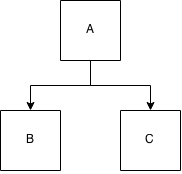
\includegraphics{pictures/cp_system.png}
  \caption{CP-system with a single master node and two slaves}
\label{cpimage}
\end{figure}

CP-systems endorse data consistency over availability. In practice this means
that when a network between two or more database nodes malfunctions, the
system should stop handling both, read and write requests from clients and wait
until the network is healed. Failure to do so might bring the systems into an
inconsistent state, where nodes of the system have different view of the same
datum. Consider figure~\ref{cpimage} that shows a CP-system consisting of a
single master node \(A\) and two slaves \(B\) and \(C\). Clients are able to
read from all of the nodes, but only node \(A\) accepts writes. After a
successful write, \(A\) replicates the write to the slave nodes. If the
connection between \(A\) and \(B\) fails, the system is partitioned into two
sets, one containing \(A\) and \(C\), and other containing only \(B\). Now if
the client first writes a new document to \(A\) and then tries to read it from
both \(B\) and \(C\), what happens is that \(C\) correctly returns the written
document, but \(B\) reports that the document can not be found. This happens
because master \(A\) was not able to replicate the new write to node \(B\)
because the network between the nodes was down. Because now \(B\) and \(C\) have
a different view of the same datum, the system can not be considered as
CP-system anymore. The situation can be fixed by not accepting a write from the
client, when the master node detects that it is not able to replicate the writes
to all nodes. 

As in the example, a common way to model CP-systems is a master/slave
architecture, where one node at a time acts as a master and other nodes are
slaves. To achieve consistency, only master is able to accept write requests and
depending on the architecture, slaves might be able to accept read requests. If
slaves handle the read requests, the distributed system might not be consistent
at all times. For example, node \(A\) accepted a write but did not had time to
replicate it to node \(B\) when it replies to the read request accessing that
object, the database would incorrectly report that object is not found. However
after \(A\) has replicated the object to \(B\) the database is again in
consistent state. This is called eventual consistency.

Vogels specifies eventual consistency as a specific form of weak
consistency\cite{vogels2009eventually}. A system with weak consistency does not
guarantee that subsequent accesses to the updated object always returns the
updated object but a set of conditions need to be met before. The period between
when the object is updated and when it is guaranteed is called
\emph{inconsistency window}.

In eventual consistency, the system guarantees that if no new updates are made
to the object, eventually all access will return the updated object. In this
case, the maximum inconsistency window in best case scenario can be calculated
from different factors of the system, such as communication delay between nodes
and the load of the system. Of course in exceptional events such as network
partition the inconsistency window can grow as large as the event occur.

The problem that many CP-systems face is what happens when the master node
becomes unavailable. That may occur for many reasons, for example the node can
suffer from hardware failure or the network between master and other nodes goes
down. Naturally the system needs to be able to recover from such cases and many
different procedures have been developed to cope with the problem. Next we
discuss how Raft consensus algorithm handles election of a new leader.

Raft is a consensus algorithm developed to replace more complex algorithm Paxos.
Raft aims to be more understandable and better uncoupled than its
predecessor\cite{chiefari1998living}. Consensus algorithms allow collection of
services to agree on some state even when some of them fails. They often arise
in context of \emph{replicated state machines}, where each service compute
identical copies of the same data. To achieve consistency, Raft selects a
distinguished leader which has a complete responsibility of managing the
replicated log and replicating them to other services. When the leader fails or
becomes unavailable, the new leader must be elected.

Raft detects leader failures with heartbeats. Each node starts as a follower and
remains in that state as long as it receives heartbeat signals from the leader.
If a follower receives no heartbeat in a period of time called \emph{election
timeout}, it assumes there are no leader and begins the leader election.

In the beginning of leader election, the follower that received no heartbeat
promotes itself to a candidate and sends vote request messages to the other
clients. A client grants the vote for the first candidate requesting the vote
and declines the rest. The candidate continues in this state until one of the
three things things happens:

\begin{enumerate}
  \item The candidate wins the election and promotes itself to the leader if it
  receives votes from majority of the cluster. Once the candidate wins the
  election it starts sending heartbeats to the other nodes and establishes the
  authority and prevents new elections.
  \item While waiting for the votes, the candidate might receive a heartbeat
  from other node. In this case it demotes itself to the follower state and
  recognizes the new leader.
  \item Last outcome is that the candidate does not win or lose the elections.
  If many followers become candidates at the same time, it is possible that none
  of the candidates receive majority of votes and initiate a new round of
  vote requests. Raft uses randomized election time outs to ensure that no two
  clients are candidates indefinitely. Another candidate might still be waiting
  out the time out when other candidate receives a majority of the votes and
  starts sending heartbeats and ending elections.
\end{enumerate}

The actual leader election in RAFT is a bit more complicated than described
above, having a concept of \emph{terms} to measure time as a logical clocks, but
they were left out for clarity. The original paper explains the election in more
detail and the website of Raft
algorithm\footnote{\url{https://raftconsensus.github.io/}} has an excellent
interactive visualization about the leader election.

\subsection{AP-systems}

\begin{figure}[h!]
  \centering
    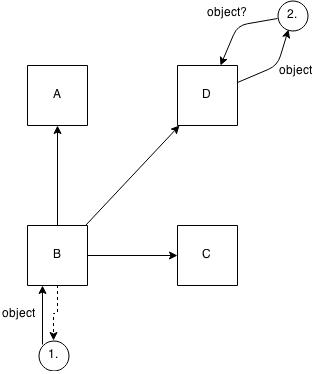
\includegraphics[scale=0.7]{pictures/ap_system.png}
  \caption{AP-system where client 1.\ sends a write request which is replicated
  to all the nodes and is read afterwards by client 2.}
\label{apimage}
\end{figure}

AP-systems choose to be available in the event of network partition instead of
keeping the data consistent at all times. In practice this means that all nodes
of the cluster are allowed to handle both read and writes requests from clients
and there is no dedicated master node. After receiving the request, the
node can either handle the request itself or delegate it to more appropriate
node for processing. Depending from the architecture, the write may be
acknowledged when the handling node has received it, or it might require
acknowledges from multiple nodes. After a successful write of an object, the
object is replicated to other nodes for a better durability and availability.
Even if a node that originally handled the write request is unavailable, the
cluster is able to respond to the request.

Figure~\ref{apimage} shows an AP-system with four nodes and two clients. First
client \(1\) sends a write request to the node \(B\) which acknowledges it
immediately, displayed as a dashed line. It then replicates the object to the
other nodes. Later client \(2\) sends a read request for the same object that
can be handled by \(D\) since it has received the object. Next consider a case
where the network is split into two different groups, client \(1\) and nodes
\(A\) and \(B\) belong to the first group and client \(2\) and nodes \(C\) and
\(D\) to second.

Because AP-systems promote availability over consistency, the system should be
able to accept writes even if the network in the cluster is malfunctioning. In
the situation of the example but with a partitioned network, client \(1\) had
sent the write request, and the write would have been acknowledged normally.
However \(B\) would have been unable to replicate the object to the nodes in the
other side of the partition and client \(2\) had got \texttt{not\_found}
response from node \(D\). This shows an important characteristics of AP-systems,
because consistency is sacrificed to obtain better availability, the service
might get into an inconsistent state but still return successful response codes
to the user. In contrast, CP-system would have rejected the write request from
\(1\) because it could not reach other nodes thus making the system unavailable.

Another interesting problem arises when a network partition heals. Assume that
both sides of the partition have received an update to the same object. Because
AP-systems do not require the write is acknowledged by majority of nodes, both
sides might end up with its own version of the same object. When the network
heals, both sides try to replicate their version to the other side but run into
a problem. Which version is correct?

Some systems solve the problem by tracking the time when an update was received
and then choosing an object with higher timestamp. This solves the problem, but
effectively destroys updates received by the other object. The system might keep
the discarded version safe so the user can try to manually merge the two
versions later. It might be tempting to try to write an universal merge function
that merges the changes from both objects in all cases. However it can be shown
that such function does not exists\todo{how is this done?}.

Because it is impossible for the AP-system to recover from all conflict cases, a
careful thought should be placed on the conflict detection. Although concurrent
updates by different clients always end up in conflict, it is possible to
automatically solve serializable updates if detected correctly. A naive way to
detect a conflict between two versions is to compare the hashes of the versions
and check whether they differ. However this approach might lead into a false
positives that can be eliminated.

Consider a case where two clients are connected to the cluster containing two
nodes. Each time a cluster receives a write request, it immediately acknowledges
it to the client and then goes to replicate it to other clients. Each node is
also allowed to handle read requests.

\begin{figure}[h!]
  \centering
    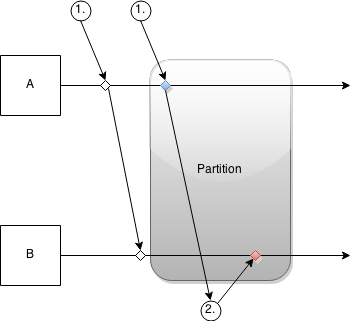
\includegraphics[scale=0.7]{pictures/apexample.png}
  \caption{Two clients updating the same object during network partition}
\label{ap-example}
\end{figure}

Figure~\ref{ap-example} presents two clients are updating the same object when a
network partition occurs.  Before the partition, client \(1\) first writes the
object which is handled by node \(A\). Node \(A\) is also able to replicate the
write to node \(B\) before the partition occurs. During the partition, client
\(1\) updates the object which handled again by node \(A\) but this time it is
not able to replicate the write to the another node. Next client \(2\) reads the
object from \(A\) and then sends an update request for that object which is
handled by \(B\). Now when the network partition heals, nodes \(A\) and \(B\)
have different versions of the same object and mark it as conflicted.

This is correct behaviour, but as we can see from the image, the conflict could
have been solved automatically. Since the writes occurred sequentially, we can
reason that the last object client \(2\) wrote to node \(B\) should be kept.
Some AP-systems, for example Amazon's Dynamo, utilize vector clocks to track
change history and to detect conflicts\cite{decandia2007dynamo}. Vector clock is
an algorithm to track partial ordering of distributed
events\cite{fidge1987timestamps}. It is consisted of a timestamp array with an
integer clock value of each process in the network. Each time the process
receives an internal event, the clock is incremented by one. Also when the array
is updated, each element is set to contain the maximum of two corresponding
values, one stored locally and one received from the sender. The value
corresponding the sender is an exception, and it is set to be one greater than
the value received, but only if the local value is not already greater than the
received value.

In practice this means that each object in the system is assigned with a vector
clock that is updated with the write request. Even during network partitions we
can keep track with vector clocks of the casual ordering and not mark sequential
writes as conflicts.

\begin{figure}[h!]
  \centering
    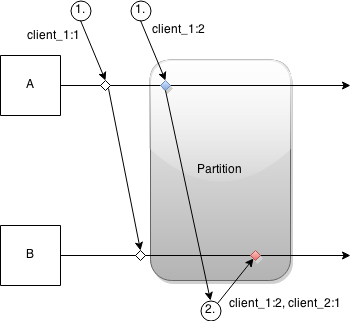
\includegraphics[scale=0.7]{pictures/apexample_clocks.png}
  \caption{Two clients updating the same object during network partition using
  vector clocks}
\label{ap-example-clocks}
\end{figure}

Figure~\ref{ap-example-clocks} shows the same example than above, but this time
the object is assigned with a vector clock. Now after the network partition is
healed, node \(A\) can tell from the vector clock that the change client \(2\)
happened to the object that was originally hold by node \(A\) and no conflict is
needed.


\section{CouchDB}

CouchDB is a distributed database that provides eventual
consistency\cite{anderson2010couchdb}. It is designed around web technologies:
it stores its documents in JSON format and all the communication internally and
externally is done over HTTP\@. CouchDB is modeled around high availability
which categorizes it as AP system.

A CouchDB cluster consists of several identical nodes running CouchDB instances.
A traditional distributed architecture has a single master node that handles all
the writes the system. Leader node then replicates these writes to several
slave nodes that can also respond to read requests by clients. Master/slave
architecture does not scale well to large scale for two reasons. First, since
all the write requests go through a single node, that node needs to have enough
processing power to handle all the request. Only way to scale to larger amount
of write requests is to scale vertically, which gets very expensive for high-end
hardware. Second, master node acts as a single point of failure in the system.
When master node fails, the distributed system can not process any write
requests until it selects a new master or the original master recovers from the
failure.

Instead of master/slave architecture, each node in CouchDB cluster acts as an
independent instance that can handle reads and writes. This enables high
availability for the cluster: even if several nodes fail, the system is still
able to process requests. However, as proven by CAP theorem, the high
availability comes with a cost: the system is no longer able to maintain
consistency between the nodes. This can affect user in certain ways, for example
user can write a document to the database and get \texttt{not\_found} error when
trying to read it moments later. This happens because database has not had time
to replicate the write operation to other node, which the user used to read the
document.

Replication in CouchDB is done asynchronously. The replication can happen
periodically or after a replication command from the user depending on the
configuration. Upon replication CouchDB compares the two databases to find out
which documents on the source differ from the target and then sends these
changes as batches until all the changes are transferred.

To find out which documents has changed, databases in CouchDB have a sequence
number which is incremented every time the database is changed. That way CouchDB
is able to tell efficiently what happened between two sequences and can send
only changed data during replication.

The client receives a successful response from the server after a single node
have processed the query. It makes no guarantees that any other node have
received or processed the query because replication takes place later. This
makes both, processing the query and replication straight forward and provides
highly available system. However, because no guarantees about replication is
made, the system can lose all the updates after last replication if the data on
the single machine is corrupted for example due a hardware failure.

It is possible to model replication differently and still have an AP system.
Riak is a distributed database that is designed based on Amazon's Dynamo
architecture\cite{decandia2007dynamo}. Riak stores objects associated with a key
to the database. It uses consistent hashing\cite{karger1997consistent} to map
the keys to the data so that single machine can acts as many virtual nodes in
the hash ring. Riak's replication is determined by multiple factors. Riak can be
configured to replicate the data up to \texttt{N} nodes in the ring, and clients
can define value \texttt{R} upon read request. Riak returns the value associated
with the key when it receives a response from \texttt{R} nodes out of \texttt{N}.
For write request the same value is called \texttt{W}. When the client sends a
write request, it can define to how many nodes Riak needs to replicate the data
to until the request is considered successful. To simulate CouchDB's behaviour,
\texttt{R=W=1} could be used, but higher values provider higher durability and
consistency.

When CouchDB database replicates updates from one server to another, it is
possible that the same document was updated in both servers. The document can
not be transferred because that would override the change that was made on the
target server. Instead, CouchDB marks the document as conflicted and
deterministically stores both versions in a way that their order is same in both
servers. Then the user is required to resolve the conflict by either choosing
one of the versions or trying to merge them.

CouchDB detects conflicts between versions by comparing \emph{revision ids} of
the documents. The database assigns revision id to each document it stores, and
it is incremented by one each time the document is updated. Because multiple
servers can update the same revision independently, the revision id also
contains a MD5 hash of the data stored in the document. If the documents have
different revision ids they are conflicting.\todo[inline]{Now there's plenty of
weird stuff here: ID is basically \texttt{<rev\_num>-MD5(document)}. Is the
algorithm able to notice consecutive edits that do not conflict and not mark
them, what about emerging branches with different revision numbers and
conflicting data?  Riak handles these with dotted version vectors, Dynamo with
vector clocks.} \todo[inline]{Should MVCC be mentioned here?}

These problems are also present in other distributed databases that allow
updates to the documents without having a consistent state of the data. This is
often true with AP systems such as Dynamo or Riak.

Dynamo tracks changes to objects using vector clocks. Each time object is
updated, it is assigned with a vector clock associated with the client that made
the change. When the updates are done concurrently and they branch, the database
can figure out the causality between the changes and automatically apply
consecutive updates. It also notices conflicts between the versions, and can
present those to user for a semantic reconciliation.

A problem with vector clocks is that the size of the clocks might grow
unbounded. If the same object is accessed with many clients, the object gets
assigned with a vector clock for each client. This takes space and slows down
algorithm detecting conflicts. For that reason, Riak has changed its conflict
resolution algorithm to use dotted version vectors\cite{preguicca2010dotted}.
Dotted version vectors work very similarly than vector clocks, but they also
include a context (called dot) where the last update was made, and the system
can safely discard earlier vectors that were seen by all parties.

Usually distributed databases are designed to store extremely large amount of
data. They achieve this by dividing the database instances to smaller partitions
called clusters. Clusters are responsible of storing and managing a portions of
the data stored in the database.

As well as Riak and Dynamo, CouchDB uses consistent hashing to determine to
which shard it routes the request. CouchDB hashes the document ID with
CRC32-based hash algorithm, and looks up from hash ring to which server the
document is stored. The hash ring mapping is stored into each proxy that handles
the requests. Because it is static, it does not automatically adapt to the
changes in the hash topology, such as removal of the node. The documentation of
CouchDB also suggests that a tree of proxies should be used for very large
clusters. The database shards are replaced with intermediate proxies that
then connect to the database shards.\todo[inline]{Manually configuration sounds
very prone to human errors, can this be included here, albeit I don't have any
references to back up my gut feeling?}

Unlike Riak, CouchDB doesn't provide a way to employ virtual nodes. With virtual
nodes, the hash ring would be split into more nodes than there are physical
servers. Also the number of nodes could be changed, and consistent hashing takes
care that no more data is moved between physical nodes than necessary. This way
the data is distributed equally between physical nodes and the cluster could be
expanded just by adding virtual nodes.

CouchDB however embraces a technique called \emph{oversharding}. In oversharding
the cluster is partitioned so that there are multiple shards in the same
physical machine. When the size of a shard grows too large, it can be moved to
the another machine or split to smaller shards. This is similar to the virtual
nodes, but the amount of shards have to be guessed before hand, and moving or
splitting shards often require human intervention, although databases with
automatic sharding exists, such as MongoDB\@\footnote{Documentation about
MongoDB sharding, including automatic sharding can be found from
http://docs.mongodb.org/manual/sharding/}.

\section{Experiment setup}

\missingfigure{Figure of the test cluster}

For the experiment, five virtual servers were deployed on the private network
using Vagrant. The servers ran Ubuntu 14.04 and CouchDB 1.5.0 was installed
using Chef.

CouchDB was installed using standard settings and each server communicated
directly with each other.

Two kinds of disturbances were simulated in the test network. First the network
was partitioned in a way, that servers 1 to 3 could not communicate with servers
4 and 5, but were able to communicate directly. Second disturbance was to slow
down the network and to cause it to lose packets.

The network partition was done using \texttt{iptables} to configure the kernel
to drop packets from corresponding servers. For example to disconnect servers 1
and 2 from rest of the cluster, following command was executed:

\begin{verbatim}
  iptables -A INPUT -s <server_host> -j DROP
\end{verbatim}

where \texttt{server\_host} was a host of the server stored in
\texttt{/etc/hosts}.

Network slowness and packet loss was caused using \texttt{tc} utility. It is a
tool used to configure Traffic Control in the Linux kernel and can be used
simulate different network problems. To configure a network interface to slow
transmission of the packets, following command was executed:

\begin{verbatim}
  tc qdisc add dev eth1 root netem delay 100ms 20ms distribution normal
\end{verbatim}

This causes \texttt{eth1} network interface to delay packets by 100ms\(\pm\)20ms
using a normal distribution. In a similar manner, packet loss was caused by
executing a following command:

\begin{verbatim}
  tc qdisc add dev eth1 root netem loss 20% 25%
\end{verbatim}

This causes \texttt{eth1} network interface to lose 20\% of packets, and each
successive probability depends by 25\% of the previous one.

The commands were executed to the servers using
Salticid\footnote{https://github.com/aphyr/salticid}. It is a relatively simple
tool used to run commands on multiple servers over SSH\@. The Salticid roles and
tasks used in the experiment are located on
GitHub\footnote{https://github.com/OsQu/couchdb-test}.

\section{Experiments}

Explain what was done and outcomes

\begin{itemize}
  \item Replication
  \item Conflicts
  \item Clustering and partitioning
  \item Consistency and Availability in Partitioned network state (i.e.\ what really happens)
  \item ACIDness (?)
  \item Load balancing (?)
\end{itemize}

\section{Conclusion}

Wrap up of the report/research. 

\begin{itemize}
  \item What was done
  \item explain results
  \item future work?
\end{itemize}


\newpage
\addcontentsline{toc}{section}{\refname}  % article

\bibliography{references.bib}
\bibliographystyle{aaltosci_t}
\end{document}
